\documentclass[tikz,border=8pt]{standalone}
% Shared look for every TikZ diagram. Load with \input{../../tools/tikz-style.tex}
\usepackage[T1]{fontenc}
\usepackage{lmodern}
\renewcommand{\sfdefault}{lmr}  % diagrams use the same serif as the text
\usetikzlibrary{arrows.meta, positioning, shapes.geometric, calc, fit, backgrounds}
\definecolor{cblue}{HTML}{4C78A8}
\definecolor{corange}{HTML}{F58518}
\definecolor{cgreen}{HTML}{54A24B}
\definecolor{cred}{HTML}{E45756}
\definecolor{cpurple}{HTML}{B279A2}
\definecolor{cgrey}{HTML}{6B6B6B}
\tikzset{
  every picture/.style={font=\sffamily, line width=1.2pt},
  box/.style={draw=#1, fill=#1!12, rounded corners=4pt, align=center, inner sep=7pt, minimum height=1.1cm},
  box/.default=cgrey,
  arrow/.style={-{Stealth[length=3mm]}, draw=cgrey, line width=1.4pt},
  title/.style={font=\sffamily\bfseries\Large},
  note/.style={font=\sffamily\small, text=cgrey, align=center},
}
\AtBeginDocument{\hyphenpenalty=10000 \exhyphenpenalty=10000}

\begin{document}
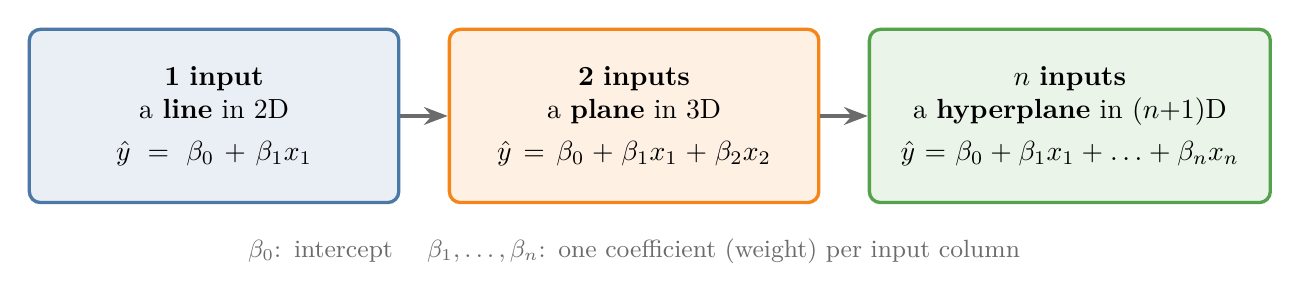
\begin{tikzpicture}[node distance=0.6cm]
  \node[box=cblue, text width=4.2cm, minimum height=2.2cm] (a) {\textbf{1 input}\\a \textbf{line} in 2D\\[3pt]$\hat{y} = \beta_0 + \beta_1 x_1$};
  \node[box=corange, text width=4.2cm, minimum height=2.2cm, right=of a] (b) {\textbf{2 inputs}\\a \textbf{plane} in 3D\\[3pt]$\hat{y} = \beta_0 + \beta_1 x_1 + \beta_2 x_2$};
  \node[box=cgreen, text width=4.6cm, minimum height=2.2cm, right=of b] (c) {\textbf{$n$ inputs}\\a \textbf{hyperplane} in $(n{+}1)$D\\[3pt]$\hat{y} = \beta_0 + \beta_1 x_1 + \dots + \beta_n x_n$};
  \draw[arrow] (a) -- (b); \draw[arrow] (b) -- (c);
  \node[note, below=0.3cm of b, text width=13cm] {$\beta_0$: intercept \quad $\beta_1, \dots, \beta_n$: one coefficient (weight) per input column};
\end{tikzpicture}
\end{document}
